
\documentclass[fleqn,addpoints]{exam}
\usepackage{amsmath}
\usepackage{graphicx}
\usepackage{booktabs}
\usepackage{float}
\usepackage{caption}
\usepackage{polynom}
\usepackage{mdwlist}
\usepackage{cancel}

\usepackage{unitsdef} 
\newunit{\inch}{in}
\newunit{\mile}{mile}
\newunit{\mph}{mph}
\newunit{\foot}{ft}
\newunit{\knot}{knot}
\newunit{\gallon}{gallon}

\bracketedpoints
\everymath{\displaystyle}

% \printanswers


% \begin{figure}[H]
%   \centering
%   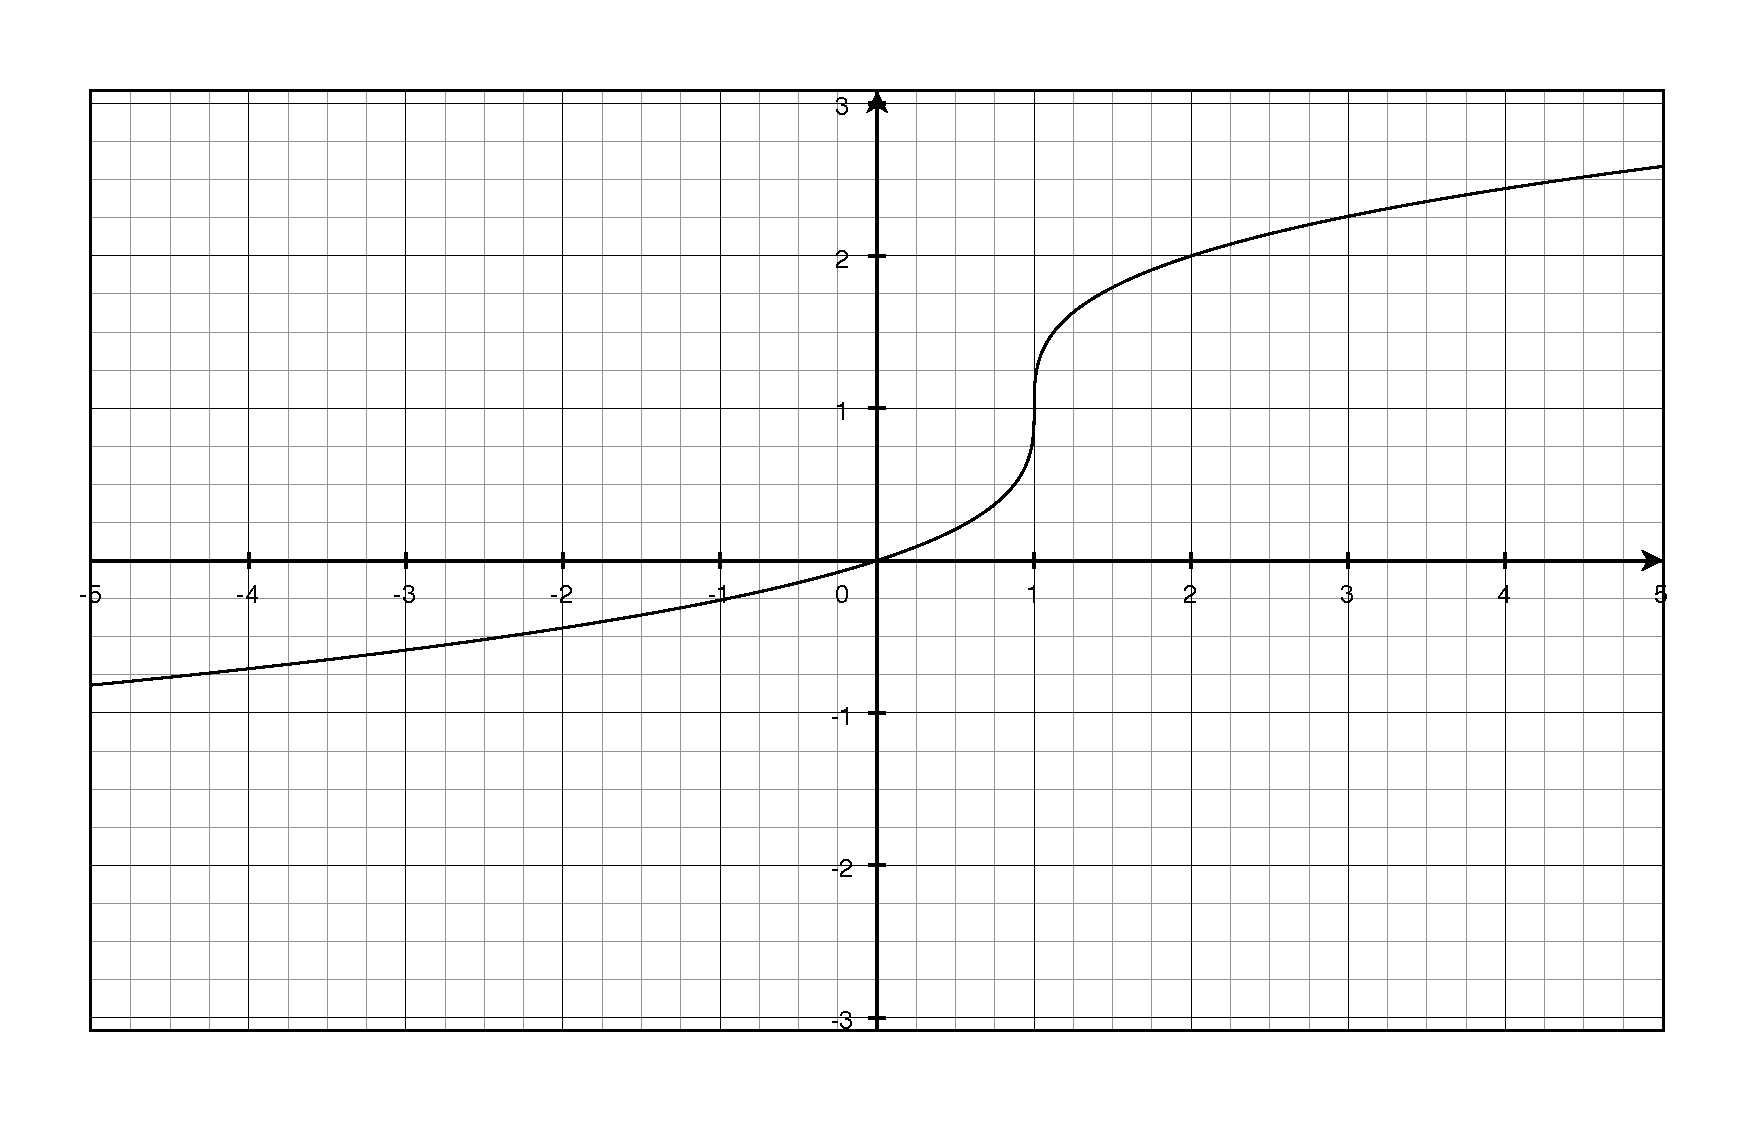
\includegraphics[scale=.3]{question7.eps}
%   \caption*{Question 7}
% \end{figure}

% \begin{tabular}{cc}
% \toprule
% period & amplitude \\
% \midrule
%   $\pi$ & $2$ \\
% \bottomrule
% \end{tabular}


\ifprintanswers
\usepackage{2in1, lscape}
\fi

\title{Math 263A Sample Final Five}

\date{November 8, 2012}

\author{}

\begin{document}

% from spring 2010 final

\maketitle  

\begin{questions}

\question
Find the limit, if it exists. $\lim_{h \to 0} \frac{(4 + h)^2 - 16}{h}$

\begin{solution}
\begin{align*}
  \lim_{h \to 0} \frac{(4 + h)^2 - 16}{h} &= \lim_{h \to 0} \frac{h^2 + 8h + 16 - 16}{h} \\
  &= \lim_{h \to 0} \frac{h(h + 8)}{h} \\
  &= \lim_{h \to 0} (h + 8) \\
  &= 8 \\
\end{align*}

\end{solution}

\question
Sketch the graph of an example of a function $f$ that satisfies all of the given conditions: 

$\lim_{x \to 0^+} = \infty$, $\lim_{x \to 0^-} = -\infty$, $\lim_{x \to \infty} = 2$, $\lim_{x \to -\infty} = -2$

\begin{solution}
  My computer can't draw these.
\end{solution}

\ifprintanswers
\pagebreak
\fi

\question
Find an equation of the tangent line to the curve at the point $\left( \pi/3, 3 \right)$. $y = 6 \cos x$

\begin{solution}
find the derivative
\[
  y' = -6 \sin x \\
\]
evaluate at $x = \frac{\pi}{3}$ to get the slope at this point:
\begin{align*}
  y' \left( \frac{\pi}{3} \right) &= -6 \sin \frac{\pi}{3} \\
  &= -3 \sqrt{3} \\
\end{align*}
find the equation of the line:
\[
  y - 3 = -3 \sqrt{3} \left(x - \frac{\pi}{3} \right)
\]
\end{solution}

\ifprintanswers
\pagebreak
\fi

\question $f(x)= \frac{3 + x}{1 - x}$
\begin{parts}
\part Find the derivative of the function using the definition of derivative. 
\begin{solution}
\begin{align*}
  f'(x) &= \lim_{h \to 0} \frac{\cfrac{3 + (x + h)}{1 - (x + h)} - \cfrac{3 + x}{1 - x}}{h} \\
        &= \lim_{h \to 0} \frac{(3 + x + h)(1 - x) - (3 + x)(1 - x - h)}{h(1 - x - h)(1 - x)} \\
        &= \lim_{h \to 0} \frac{4 \cancel{h}}{\cancel{h}(1 - x - h)(1 - x)} \\
        &= \lim_{h \to 0} \frac{4}{(1 - x - h)(1 - x)} \\
        &= \frac{4}{(1 - x)^2} \\
\end{align*}

\end{solution}

\part Check your answer using differentiation rules. 
\begin{solution}
\begin{align*}
  f'(x) &= \frac{(1 - x) - (3 + x)(-1)}{(1 - x)^2} \\
        &= \frac{4}{(1 - x)^2} \\
\end{align*}
\end{solution}

\part State the domain of the function and the domain of the derivative.  
\begin{solution}
  For both, the domain is $x \neq 1$
\end{solution}

\end{parts}

\ifprintanswers
\pagebreak
\fi

\question
Find the derivative of the function $y = \sin \left( \sqrt{1 + x^2} \right)$

\begin{solution}

Apply the chain rule twice:
\begin{align*}
  y &= \sin (1 + x^2)^{1/2} \\
  y' &= \cos(1 + x^2)^{1/2} \cdot D_x (1 + x^2)^{1/2} \\
     &= \cos(1 + x^2)^{1/2} \frac{1}{2} (1 + x^2)^{-1/2} \cdot D_x (1 + x^2) \\
     &= \cos(1 + x^2)^{1/2} \cdot \frac{1}{2}(1 + x^2)^{-1/2} \cdot 2x \\
     &= \frac{x \cos \left( \sqrt{1 + x^2} \right)}{\sqrt{1 + x^2}} \\
\end{align*}

\end{solution}

\question
Find the derivatives of the functions:
\begin{parts}
\part $y = \sqrt[4]{1 + 2x + x^3}$
\begin{solution}
\begin{align*}
  y &= (1 + 2x + x^3)^{1/4} \\
  y' &= \frac{1}{4} (1 + 2x + x^3)^{-3/4} \cdot (2 + 3x^2) \\
     &= \frac{2 + 3x^2}{4 (1 + 2x + x^3)^{3/4}} \\
\end{align*}

\end{solution}

\ifprintanswers
\pagebreak
\fi

\part $y = \frac{3x - 1}{2x + 1}$
\begin{solution}
\begin{align*}
  y &= \frac{3x - 1}{2x + 1} \\
  y' &= \frac{(2x + 1)3 - (3x - 1)2}{(2x + 1)^2} \\
     &= \frac{6x + 3 - 6x + 2}{(2x + 1)^2} \\
     &= \frac{5}{(2x + 1)^2} \\
\end{align*}

\end{solution}

\end{parts}

\question
Find $\frac{dy}{dx}$ by implicit differentiation and simplify if possible. 
\[
  \tan(xy) = x + y
\]

\begin{solution}
\begin{align*}
  \tan(xy) &= x + y \\
  \sec^2(xy) \cdot D_x (xy) &= 1 + y' \\
  \sec^2(xy) \cdot (xy' + y) &= 1 + y' \\
  y' &= \frac{1 - y \sec^2(xy)}{x \sec^2(xy) - 1}
\end{align*}

\end{solution}

\ifprintanswers
\pagebreak
\fi

\question 
Two cars start moving from the same point at the same time. One travels south at $60 \mph$ and the other travels west at
$25 \mph$. At what rate is the distance between the cars increasing two hours later?

\begin{solution}
The distance between the cars is: $r^2 = x^2 + y^2$.  Differentiate with respect to time and solve for $\frac{dr}{dt}$:
\[
  \frac{dr}{dt} = \frac{x}{r} \cdot \frac{dx}{dt} + \frac{y}{r} \cdot \frac{dy}{dt}
\]
at the time we're interested in, the numbers are:
\begin{align*}
  \frac{dx}{dt} &= -25 \mph \\
  \frac{dy}{dt} &= -120 \mph \\
  x &= -50 \mile \\
  y &= -120 \mile \\
  r &= 130 \mile \\
\end{align*}
plug all these numbers in to get the answer: 
\[
  \frac{dr}{dt} = 65 \mph
\]

\end{solution}

\ifprintanswers
\pagebreak
\fi

\question Find the dimensions of the rectangle of largest area that has its base on the x-axis and its other vertices
above the x-axis and lying on the parabola $y = 8 - x^2$.

\begin{solution}
If the bottom of the rectangle goes from $-x$ to $x$, the area of the rectangle is: $A = 2xy$.  We need an equation which only contains $x$:
\begin{align*}
  A &= 2xy \\
    &= 2x(8 - x^2) \\
    &= 16x - 2x^3 \\
\end{align*}
differentiate:
\[
  A'(x) = 16 - 6x^2 
\]
find critical points:
\begin{align*}
  16 - 6x^2 &= 0 \\
  x &= \sqrt{\frac{8}{3}} \\
\end{align*}
plug back in to find $y$:
\begin{align*}
  y &= 8 - x^2 \\
    &= \frac{16}{3} \\
\end{align*}
\end{solution}

\ifprintanswers
\pagebreak
\fi

\question
Find the limit. 
\[
  \lim_{x \to -2} \frac{x^2 - 1}{x + 1}
\]

\begin{solution}
\begin{align*}
  \lim_{x \to -2} \frac{x^2 - 1}{x + 1} &= \lim_{x \to -2} \frac{\cancel{(x + 1)}(x - 1)}{\cancel{x + 1}} \\
  &= \lim_{x \to -2} (x - 1) \\
  &= -3 \\
\end{align*}
\end{solution}

\ifprintanswers
\pagebreak
\fi

\question
Find the local maximum and local minimum values of $f$ using either the First or Second Derivative Tests.
\[
  f(x) = x + \sqrt{1 - x}
\]

\begin{solution}

find the derivatives:
\begin{align*}
  f(x) &= x + (1 - x)^{1/2} \\
  f'(x) &= 1 + \frac{1}{2}(1 - x)^{-1/2}(-1) \\
        &= 1 - \frac{1}{2}(1 - x)^{-1/2} \\
        &= 1 - \frac{1}{2 \sqrt{1 - x}} \\
  f''(x) &= \frac{1}{4}(1 - x)^{-3/2}(-1) \\
         &= -\frac{1}{4}(1 - x)^{-3/2} \\
         &= -\frac{1}{4(1 - x)^{3/2}} \\
\end{align*}

find the critical points:
\begin{align*}
  1 - \frac{1}{2 \sqrt{1 - x}} &= 0 \\
  \frac{1}{2 \sqrt{1 - x}} &= 1 \\
  % 2 \sqrt{1 - x} &= 1 \\
  \sqrt{1 - x} &= \frac{1}{2} \\
  1 - x &= \frac{1}{4} \\
  x &= \frac{3}{4} \\
\end{align*}

Since the second derivative is always negative, this is a maximum value and there aren't any minimum values.

So the maximum is: $\left(\frac{3}{4}, \frac{5}{4} \right)$

\end{solution}

\question
The volume of a cube is increasing at a rate of $10 \centimeter^3 / \minute$.  How fast is the surface area increasing
when the length of an edge is $30 \centimeter$?

\begin{solution}

If the length of a side is $x$, the two equations we know are:
\begin{align*}
  V &= x^3 \\
  A &= 6x^2 \\
\end{align*}

{\em approach 1}

differentiate both equations with respect to time:
\begin{align*}
  \frac{dV}{dt} &= 3x^2 \cdot \frac{dx}{dt} \\
  \frac{dA}{dt} &= 12x \cdot \frac{dx}{dt} \\
\end{align*}

since we have $\frac{dV}{dt}$ and we want $\frac{dA}{dt}$, we need to get rid of $\frac{dx}{dt}$:
\begin{align*}
  \frac{dV}{dt} &= 3x^2 \cdot \frac{dx}{dt} \\
  \frac{dx}{dt} &= \frac{1}{3x^2} \cdot \frac{dV}{dt} \\
\\
  \frac{dA}{dt} &= 12x \cdot \frac{1}{3x^2} \cdot \frac{dV}{dt} \\
    &= \frac{4}{x} \cdot \frac{dV}{dt} \\
\end{align*}

\ifprintanswers
\pagebreak
\fi

{\em approach 2}

find the area in terms of the volume:
\begin{align*}
  x &= V^{1/3} \\
  A &= 6 \left(V^{1/3} \right)^2 \\
    &= 6 V^{2/3} \\
\end{align*}

differentiate
\begin{align*}
  \frac{dA}{dt} &= 4 \cdot V^{-1/3} \cdot \frac{dV}{dt} \\
                &= \frac{4}{\sqrt[3]{V}} \cdot \frac{dV}{dt} \\
                &= \frac{4}{x} \cdot \frac{dV}{dt} \\
\end{align*}

Either way (approach 1 or approach 2), we can now can plug in the values to get the answer:
\begin{align*}
  \frac{dA}{dt} &= \frac{4}{30} \cdot 10 \\
  &= \frac{4}{3} \cm^2 / \min \\
\end{align*}

\end{solution}

\ifprintanswers
\pagebreak
\fi

\question $f(x) = x^4 + 4x^3$

\begin{parts}
\part Find the vertical and horizontal asymptotes, if any.
\begin{solution}
  Since this function is a polynomial, there aren't any asymptotes.
\end{solution}

\part Find the intervals on which $f$ is increasing or decreasing. 
\begin{solution}
differentiate:
\[
  f'(x) = 4x^3 + 12x^2
\]
find the critical points:
\begin{align*}
  4x^3 + 12x^2 &= 0 \\
  x^2(x + 3) &= 0 \\
  x &= \{-3, 0\} \\
\end{align*}

use a sign chart or sample points to find where the function is increasing and decreasing:
\begin{itemize*}
\item decreasing: $(-\infty, -3)$
\item increasing: $(-3, 0) \cup (0, \infty)$
\end{itemize*}

\end{solution}

\part Find the local maximum and minimum values of $f$.
\begin{solution}
  From part (b), you can see that there is a minimum at $(-3, -27)$ and no maximum.
\end{solution}

\part Find the intervals of concavity and the inflection points. 
\begin{solution}
find the second derivative
\[
  f''(x) = 12x^2 + 24x
\]
find the inflection points:
\begin{align*}
  12x^2 + 24x &= 0 \\
  x(x + 2) &= 0 \\
  x &= \{-2, 0\} \\
\end{align*}
use a sign chart or sample points to find where the function is concave up/down:
\begin{itemize*}
\item concave up: $(-\infty, -2) \cup (0, \infty)$
\item concave down: $(-2, 0)$
\end{itemize*}

\end{solution}

\part Use the information from (a) - (d) to sketch the graph.
\begin{solution}
\begin{figure}[H]
  \centering
  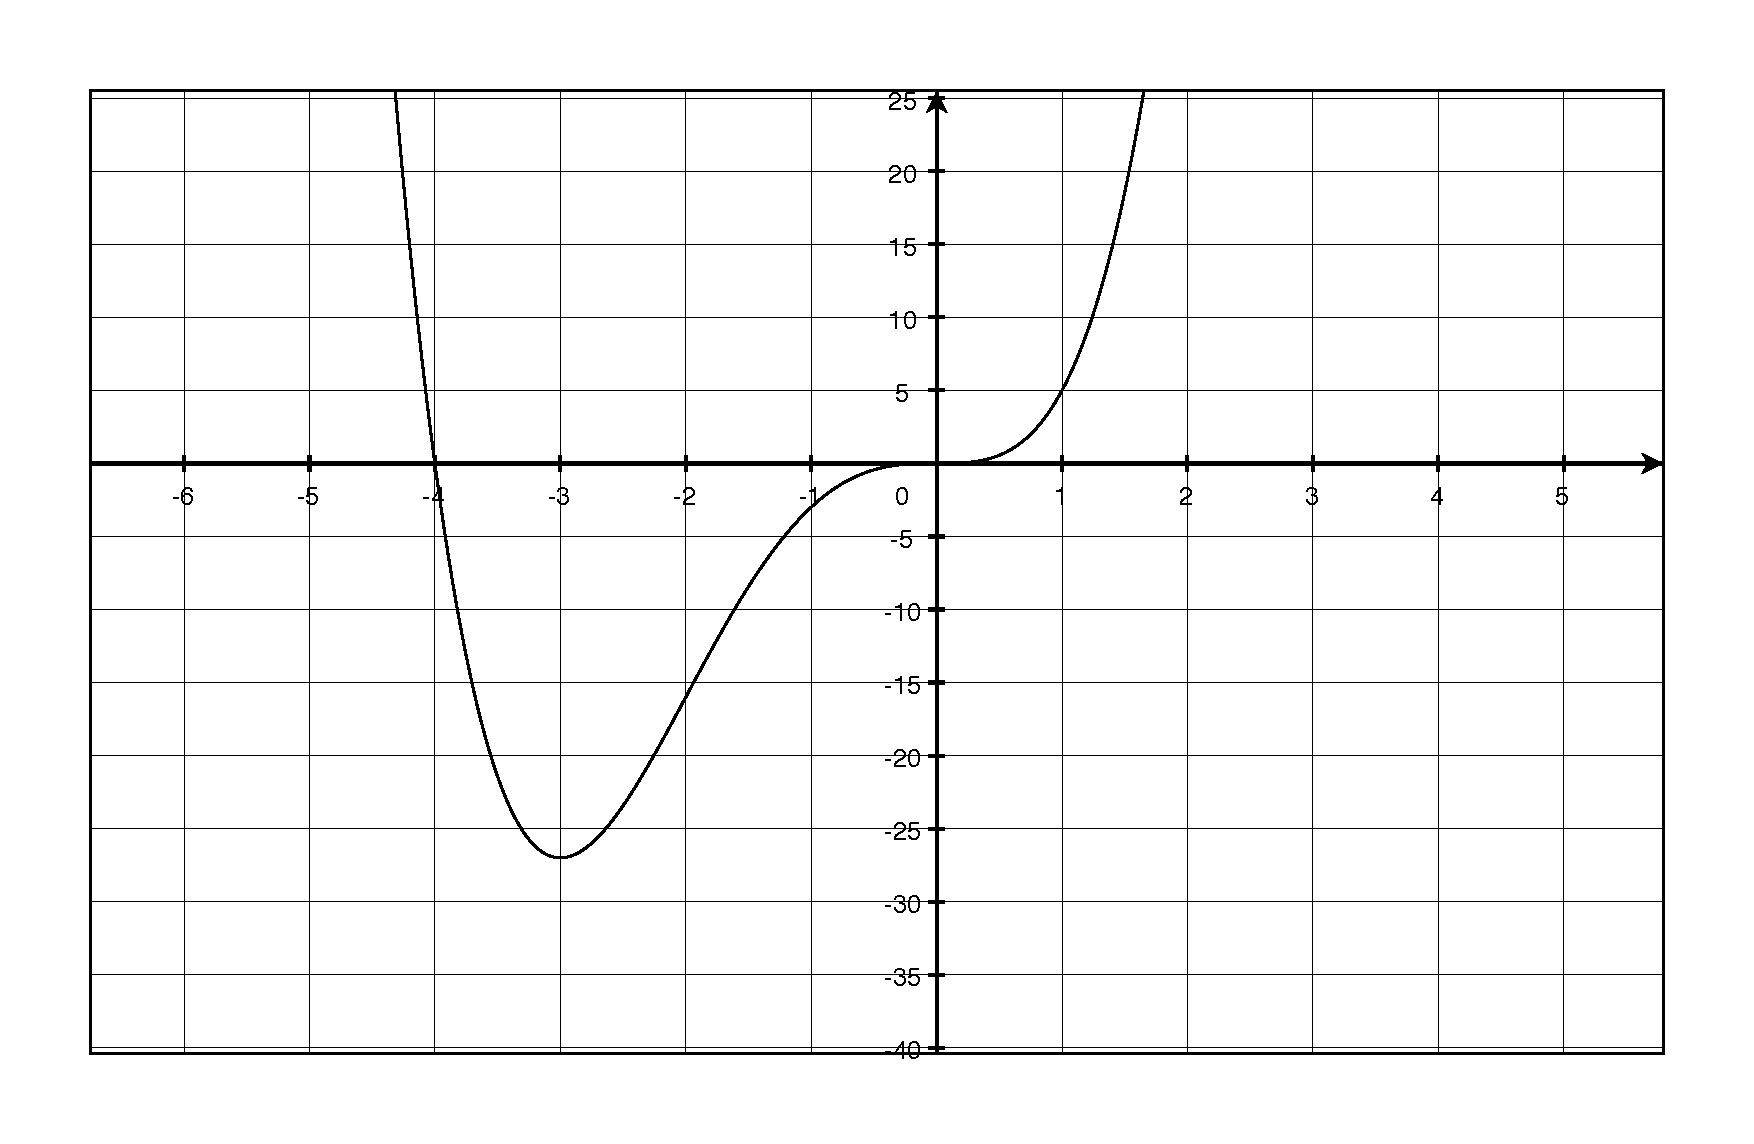
\includegraphics[scale=.3]{final_5_q14.eps}
  \caption*{Question 14}
\end{figure}
\end{solution}

\end{parts}


\end{questions}

\end{document}
